\chapter{Image import}

InVesalius imports files in DICOM format, including compressed files (lossless JPEG), Analyze (Mayo Clinic$^\copyright$), NIfTI, PAR/REC, BMP, TIFF, JPEG and PNG formats.

\section{DICOM}

Under the File menu, click on Import DICOM or use the shortcut Ctrl+I. Additionally, DICOM files can be imported by clicking on the icon shown in Figure~\ref{fig:import}.

\begin{figure}[!htb]
\centering

\includegraphics[scale=0.2]{../user_guide_figures/icons/file_import_original.png}
\caption{Shortcut to DICOM import}
\label{fig:import}
\end{figure}

\hspace{.2cm}

Select the directory containing the DICOM files, as in Figure~\ref{fig:win_folder}. InVesalius will search for files also in subdirectories of the chosen directory,
if they exist.

\newpage

Once the directory is selected, click \textbf{OK}.

\begin{figure}[!htb]
\centering
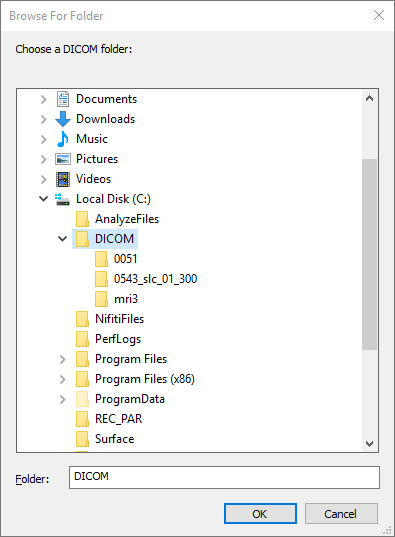
\includegraphics[scale=0.5]{../user_guide_figures/invesalius_screen/import_select_folder_en.png}
\caption{Folder Selection}
\label{fig:win_folder}
\end{figure}

\hspace{.2cm}

While InVesalius search for DICOM files in the directory, the loading progress of the scanned files is displayed, as shown in the Figure~\ref{fig:ver_file}.

\begin{figure}[!htb]
\centering
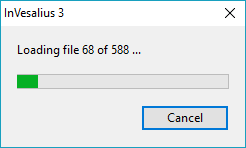
\includegraphics[scale=0.6]{../user_guide_figures/invesalius_screen/import_load_files_en.png}
\caption{Loading file status}
\label{fig:ver_file}
\end{figure}

\newpage

If DICOM files are found, a window open (shown Figure~\ref{fig:win_import}) will open to select the patient and respective series to be opened. It is also possible to skip images for reconstruction.

\begin{figure}[!htb]
\centering
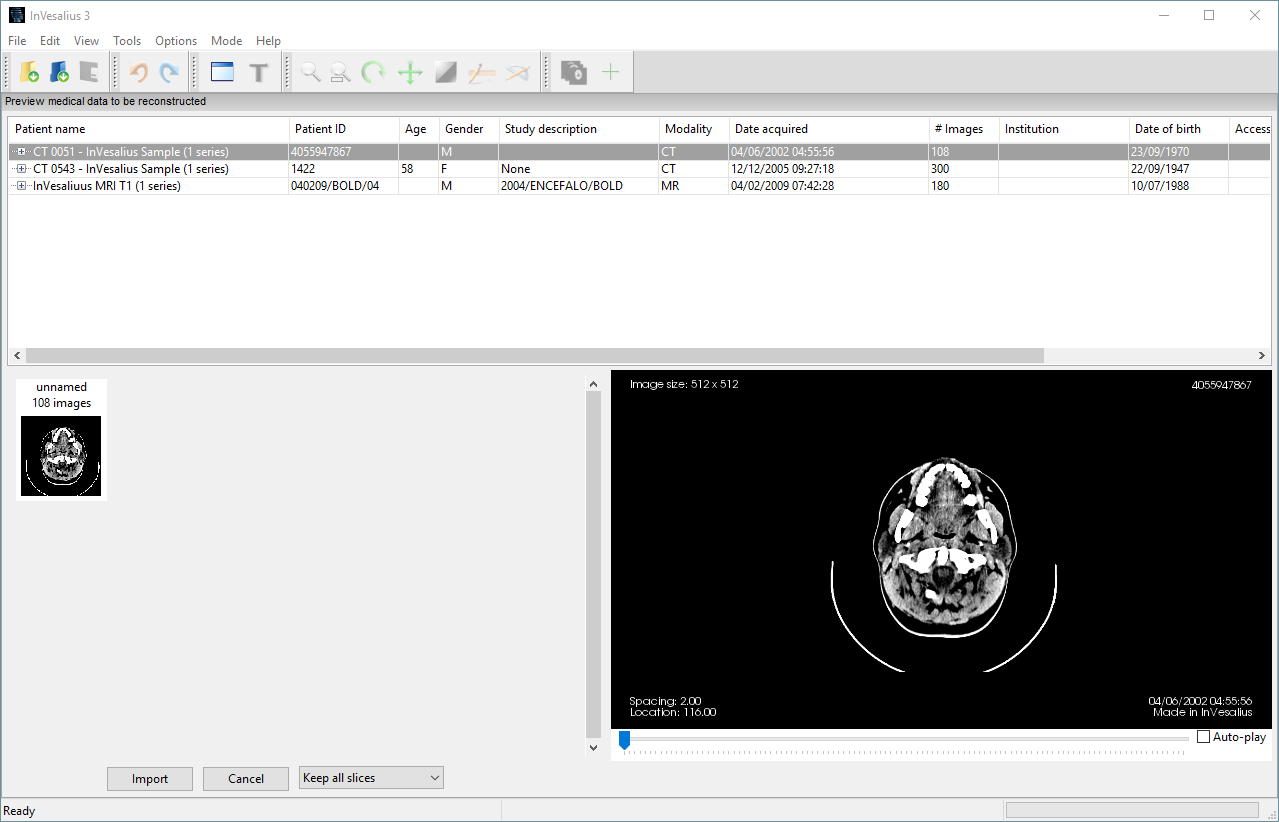
\includegraphics[scale=0.4]{../user_guide_figures/invesalius_screen/import_window_en.png}
\caption{Import window}
\label{fig:win_import}
\end{figure}

\newpage

To import a series with all images present, click "\textbf{$+$}" on the patient’s name to expand the corresponding series. Double-click on the description of the series. See Figure~\ref{fig:import_serie}.

\begin{figure}[!htb]
\centering
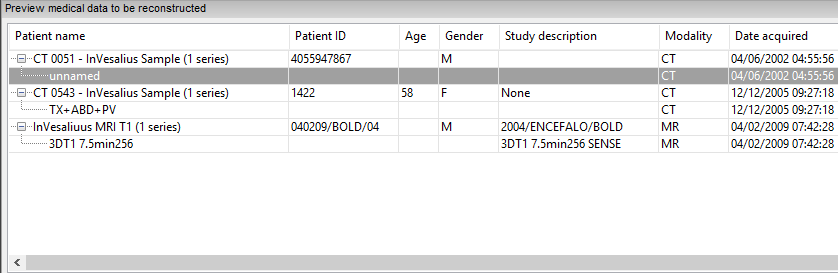
\includegraphics[scale=0.5]{../user_guide_figures/invesalius_screen/import_window_detail_en.png}
\caption{Series selection}
\label{fig:import_serie}
\end{figure}

In some cases, when there is no computer with memory and/or satisfactory processing to work with large numbers of images in a series, it is recommended to skip some of them. To do this, click \textbf{once} with the \textbf{left} mouse button over the description of the series (Figure~\ref{fig:import_serie}) and select how many images will be skipped (Figure~\ref{fig:skip_image}), then click \textbf{Import}.

\begin{figure}[!htb]
\centering
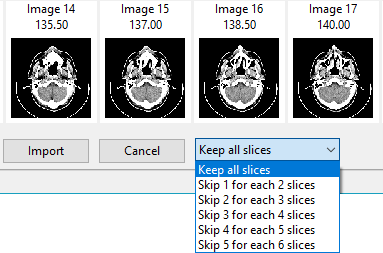
\includegraphics[scale=0.6]{../user_guide_figures/invesalius_screen/import_window_skip_slice_en.png}
\caption{Skip imagens option}
\label{fig:skip_image}
\end{figure}

If there is an insufficient amount of available memory at the time of loading the images it is recommended that the resolution of the slices be reduced to work with volumetric and surface visualization, as shown in Figure~\ref{fig:resize_image}.
The slices will be resized according to the percentage relative to the original resolution. For example, if each slice of the exam the dimension of 512 x 512 pixels and the "Percentage of original resolution" is suggested to be 60 \%, each resulting image will be 307 x 307 pixels. To open with the original pixel resolution, set the percentage to 100.

\begin{figure}[!htb]
\centering
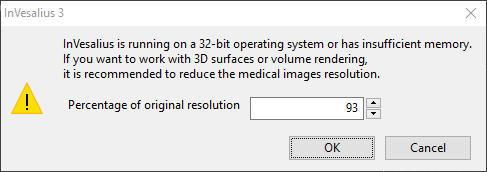
\includegraphics[scale=0.5]{../user_guide_figures/invesalius_screen/import_window_lower_memory_en.png}
\caption{Image size reduction}
\label{fig:resize_image}
\end{figure}

If the image was obtained with the gantry tilted it will be necessary to correct to avoid distortion of any reconstruction. InVesalius allows the user to do this easily. When importing an image with the gantry tilted a dialog will appear, showing the gantry tilt angle. (Figure~\ref{fig:gantry_tilt}). It is possible to change this value, but it is not recommended. Click on the \textbf{Ok} to do the correction. If you click on the \textbf{cancel} button the correction will not be done.

\begin{figure}[!htb]
\centering
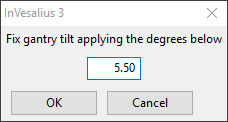
\includegraphics[scale=0.75]{../user_guide_figures/invesalius_screen/window_gantry_tilt_en.png}
\caption{Gantry tilt correction}
\label{fig:gantry_tilt}
\end{figure}

After the above procedure, a window will be displayed (Figure \ref{fig:prog_recons}) with reconstruction (when images are stacked and interpolated).

\begin{figure}[!htb]
\centering
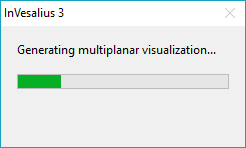
\includegraphics[scale=0.6]{../user_guide_figures/invesalius_screen/import_window_progress_en.png} 
\caption{Reconstruction progress}
\label{fig:prog_recons}
\end{figure}

\newpage

\section{Analyze}

To import Analyze files, under the \textbf{File} menu, click \textbf{Import other files}, then click in the \textbf{Analyze} option as show the Figure~\ref{fig:analyze_menu}.

\begin{figure}[!htb]
\centering
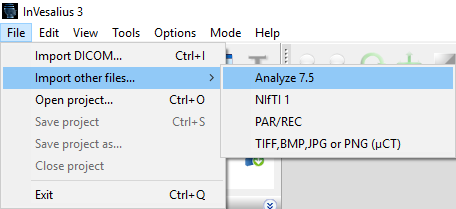
\includegraphics[scale=0.4]{../user_guide_figures/invesalius_screen/import_analyze_menu_en.png}
\caption{Menu for importing images in analyze format.}
\label{fig:analyze_menu}
\end{figure}

Select the Analyze file format (\textbf{.hdr}) and click on \textbf{Open} (Figure~\ref{fig:analyze_import}).
 
\begin{figure}[!htb]
\centering
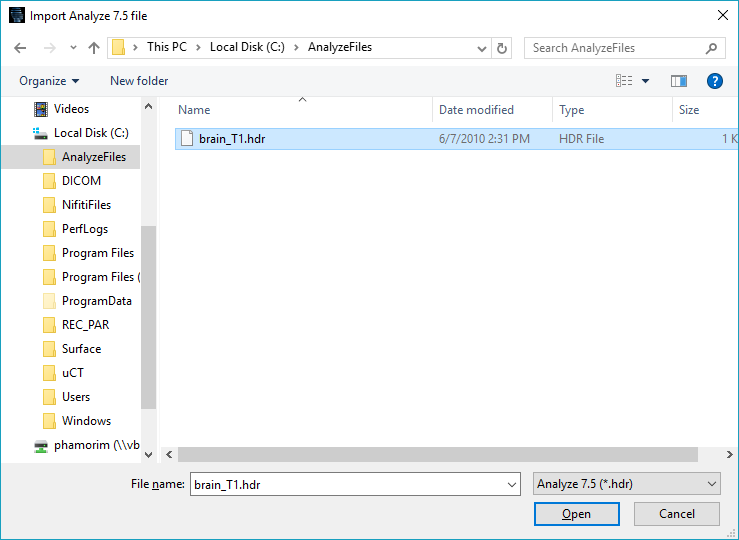
\includegraphics[scale=0.4]{../user_guide_figures/invesalius_screen/import_analyze_window_en.png}
\caption{Import analyze file format}
\label{fig:analyze_import}
\end{figure}

\section{NIfTI}

To import NIfTI files, under the \textbf{File}  menu, click \textbf{Import other files} and then click \textbf{NIfTI} as shown in Figure~\ref{fig:import_nifti_menu_pt}.


\begin{figure}[!htb]
\centering
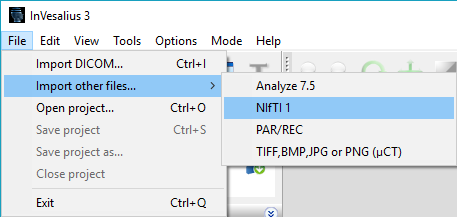
\includegraphics[scale=0.4]{../user_guide_figures/invesalius_screen/import_nifti_menu_en.png}
\caption{Menu to import images in NIfTI format}
\label{fig:import_nifti_menu_pt}
\end{figure}

Select the NIfTI file format, (either \textbf{nii.gz} or \textbf{.nii}) then click \textbf{Open} (Figure~\ref{fig:import_nifti_window_pt}). If the file is in another format as \textbf{.hdr}, select \textbf{all files(*.*)} option.

\begin{figure}[!htb]
\centering
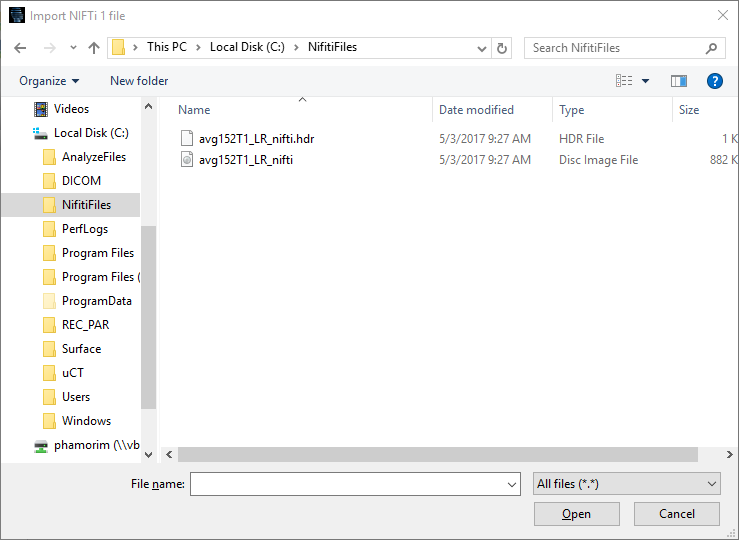
\includegraphics[scale=0.4]{../user_guide_figures/invesalius_screen/import_nifti_window_en.png}
\caption{Importing images in NIfTI format.}
\label{fig:import_nifti_window_pt}
\end{figure}

\section{PAR/REC}

To import PAR/REC file, under the \textbf{File} menu, click \textbf{Import other files}, and then click on \textbf{PAR/REC} as shown in Figure~\ref{fig:import_parrec_menu_pt}.

\begin{figure}[!htb]
\centering
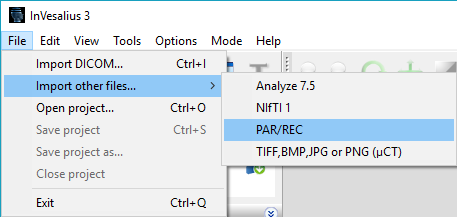
\includegraphics[scale=0.4]{../user_guide_figures/invesalius_screen/import_parrec_menu_en.png}
\caption{Menu for importing PAR/REC images}
\label{fig:import_parrec_menu_pt}
\end{figure}

Select PAR/REC file type, with the file extension \textbf{.par} and click \textbf{Open} (Figure~\ref{fig:import_parrec_window_pt}). If the file has no extension, select \textbf{all files(*.*)} option.

\begin{figure}[!htb]
\centering
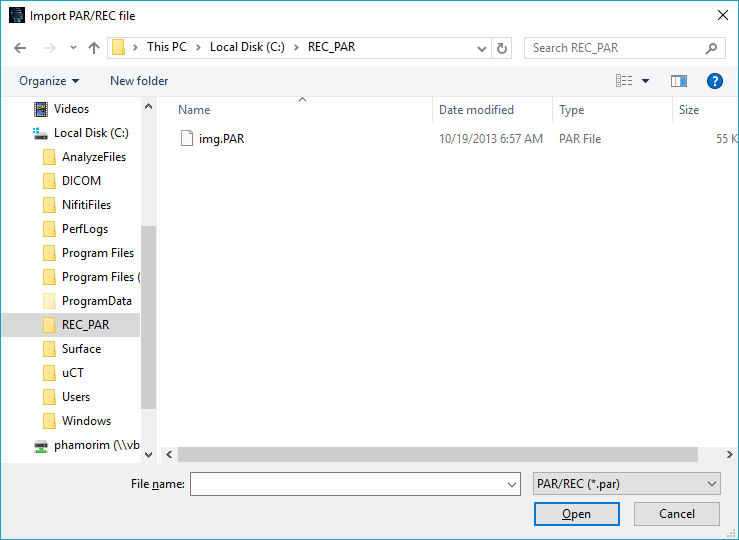
\includegraphics[scale=0.4]{../user_guide_figures/invesalius_screen/import_parrec_window_en.png}
\caption{PAR/REC import}
\label{fig:import_parrec_window_pt}
\end{figure}

\section{TIFF, JPG, BMP, JPEG or PNG (micro-CT)}

TIFF, JPG, BMP, JPEG or PNG file format for microtomography equipment (micro-CT or $\mu$CT) or others. InVesalius imports files in these formats if pixels present are represented in \textbf{grayscale}.

To import, click on menu \textbf{File}, \textbf{Import other files...} and then click on \textbf{TIFF, JPG, BMP, JPEG ou PNG ($\mu$CT)} option as shown the figure~\ref{fig:import_bmp_menu_pt}.

\begin{figure}[!htb]
\centering
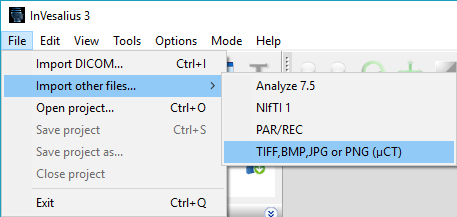
\includegraphics[scale=0.4]{../user_guide_figures/invesalius_screen/import_bmp_menu_en.png}
\caption{Import images in BMP and others formats}
\label{fig:import_bmp_menu_pt}
\end{figure}

Select the directory that contains the files, as shown the Figure~\ref{fig:import_bmp_select_folder}. InVesalius will search for files also in subdirectories of the chosen directory, if they exist. 

Click on \textbf{OK}.

\begin{figure}[!htb]
\centering
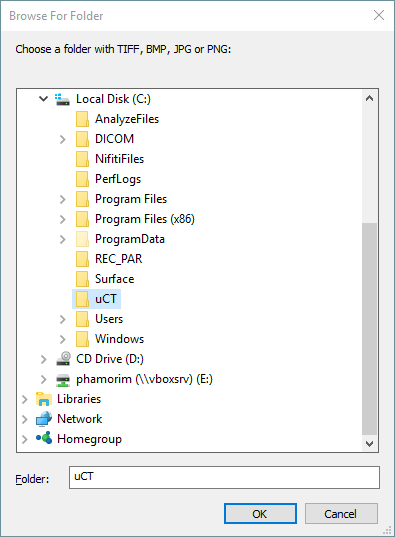
\includegraphics[scale=0.5]{../user_guide_figures/invesalius_screen/import_bmp_select_folder_en.png}
\caption{Folder selection}
\label{fig:import_bmp_select_folder}
\end{figure}

While InVesalius is looking for TIFF, JPG, BMP, JPEG, or PNG files in the directory, the upload progress of the scanned files is displayed, as illustrated in Figure~\ref{fig:import_bmp_load_pt}.

\begin{figure}[!htb]
\centering
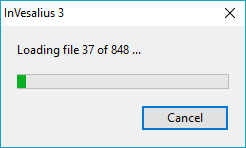
\includegraphics[scale=0.6]{../user_guide_figures/invesalius_screen/import_bmp_load_en.png}
\caption{Checking and loading files status.}
\label{fig:import_bmp_load_pt}
\end{figure}

If files in the desired formats are located, a window will open (shown in Figure~\ref{fig:import_bmp_window_pt}) to display the files eligible for reconstruction. Images can also be skipped to remove files from the rebuild list. The files are sorted according to file names. It is recommended that the files are numbered according to the desired rebuild order.

\begin{figure}[!htb]
\centering
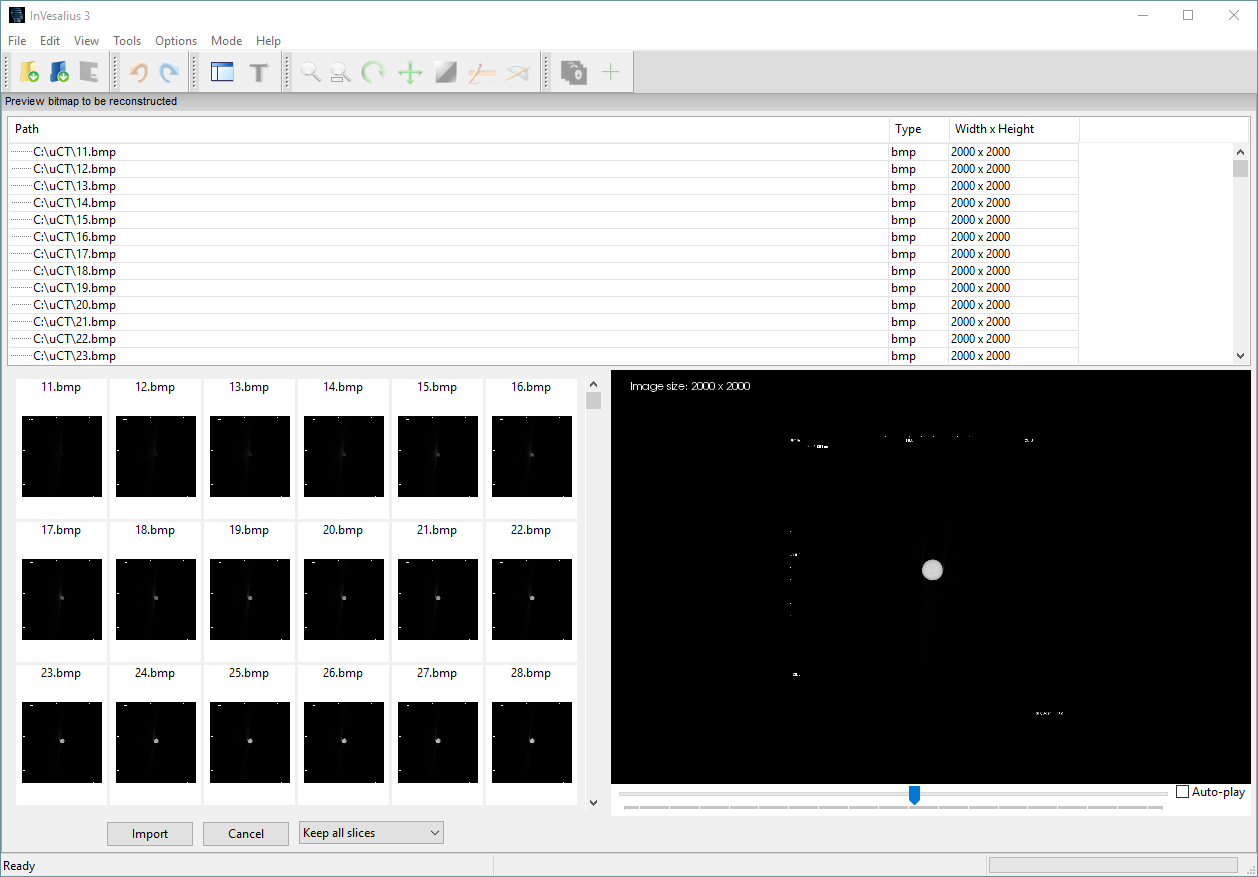
\includegraphics[scale=0.3]{../user_guide_figures/invesalius_screen/import_bmp_window_en.png}
\caption{Window to import BMP files.}
\label{fig:import_bmp_window_pt}
\end{figure}
 
To delete files that are not of interest, select a file by clicking the left mouse button and then pressing the delete key. You can also choose a
range of files to delete by clicking the \textbf{left mouse button} on a file, holding down the \textbf{shift} key, clicking again with the mouse button in the last file of the track and finally pressing the \textbf{delete} button.

Similar to when importing DICOM files, you can skip BMP images for re-building. In some cases, particularly where a computer with satisfactory memory and/or processing is unavailable, it may be advisable to skip some of them to retain adequate program functionality. To do this, select how many images to skip (Figure~\ref{fig:import_bmp_skip_pt}), then click \textbf{Import}.

\begin{figure}[!htb]
\centering
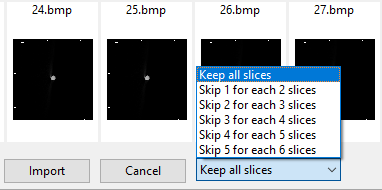
\includegraphics[scale=0.4]{../user_guide_figures/invesalius_screen/import_bmp_skip_en.png}
\caption{Importation window}
\label{fig:import_bmp_skip_pt}
\end{figure}

To reconstruct files of this type, a project name must be defined to indicate the orientation of the images (axial, coronal or sagittal), voxel spacing ($X$, $Y$ and $Z$) in \textbf{mm} as shown in the Figure~\ref{fig:import_bmp_spacing_pt}. The voxel spacing in $X$ is the pixel width of each image, $Y$ the pixel length, and $Z$ represents the distance of each slice (voxel height).

If the image set consists of microtomography images, more specifically GE and Brucker equipment, it is possible that InVesalius will read the text file with the acquisition parameters that normally stay in the same folder as the images and automatically insert the spacing. This verification can be done when the values of $X$, $Y$ and $Z$ are different from "1.00000000", otherwise it is necessary to enter the values of the respective spacing.

\textbf{Correct spacing is crucial for correctly importing objects in InVesalius. Incorrect spacing will provide incorrect measurements.}

Once all parameters have been input, click \textbf{OK}.

\begin{figure}[!htb]
\centering
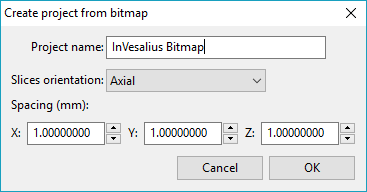
\includegraphics[scale=0.5]{../user_guide_figures/invesalius_screen/import_bmp_spacing_en.png}
\caption{Import Screen}
\label{fig:import_bmp_spacing_pt}
\end{figure}

If insufficient memory is available when loading images, it is recommended to reduce the resolution of the slices to work with volumetric and surface visualization, as shown in Figure~\ref{fig:import_bmp_resize_pt} window.The slices will be resized according to the percentage relative to the original resolution. For example, if each slice of the exam contains the dimension of $512 x 512$ pixels and the "Percentage of the original resolution" is suggested at 60, each resulting image will have $307 x 307$ pixels. If you want to open with the original resolution set the percentage to $100$.

\begin{figure}[!htb]
\centering
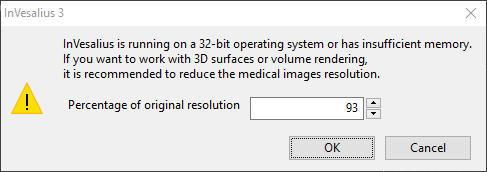
\includegraphics[scale=0.5]{../user_guide_figures/invesalius_screen/import_window_lower_memory_en.png}
\caption{Image resize}
\label{fig:import_bmp_resize_pt}
\end{figure}

After the previous steps, wait a moment for the program to complete the multiplanar reconstruction as shown in Figure~\ref{fig:import_bmp_mpr_pt.png}.

\begin{figure}[!htb]
\centering
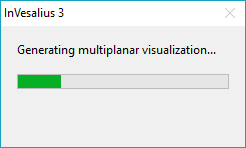
\includegraphics[scale=0.6]{../user_guide_figures/invesalius_screen/import_window_progress_en.png}
\caption{Multiplanar reconstruction in progress.}
\label{fig:import_bmp_mpr_pt.png}
\end{figure}
